\documentclass[12pt]{article}
\usepackage{enumerate}
\usepackage{mathematics}

\begin{document}

\title{Visual Group Theory}
\author{}
\date{}
\maketitle

\begin{enumerate}
\item Group is a set of actions
\item Define group with a set of simple actions (``moves'') -- these are the {\bf generator}
  actions for the group.
\item Any sequence of generator actions is another action in the group.
\item Note that the starting state is arbitrary: to solve a Rubik's cube means to find the inverse
  of a given \emph{sequence of actions}. Not to find the ``inverse of a state''.
\item A Cayley diagram is a graph in which the nodes are actions, and the edges are generators. An
  assignment of state (e.g. a labeled shape in space) to one node, implies the states at all other
  nodes.
\end{enumerate}

\section{}
\begin{enumerate}
\item[1] {\bf Two coins, only action is transposition. Is that a group?}\\
  With identity, then yes, $\{e, \tau\}$ is associative, has inverses and is closed. \checkmark
\item[3] {\bf Transferring marbles between pockets:}\\
  Not a group, some sequences of actions are impossible due to the statefulness. \checkmark
\item[5] {\bf Does closure mean infinitely many actions?}\\
  No. Infinitely many sequences of actions but only finitely many distinct actions (for a finite
  group). \checkmark
\item[7] {\bf (a) Transposition twice in a row:}\\
  $e$. \checkmark
\item[10] {\bf Finite group-like object lacking inverses:}\\
  Any non-reversible action - \checkmark
\item[12] {\bf Finite non-closed group-like object:}\\
  Actions changing a stateful object that can't be indefinitely chained - \checkmark
\end{enumerate}


\section{}
\begin{enumerate}
\item[1] {\bf rectange}\\
  generators are horizontal and vertical reflections; other element is their product. \checkmark
\item[3] {\bf Can an arrow in a Cayley diagram ever connect a node to itself?}\\
  No, an arrow corresponds to applying a generator action; the identity is not a generator of any
  group other than $\{e\}$, but in that case there would be no arrow. \checkmark
\item[4] {\bf Two coins, only action is transposition. Create Cayley diagram}\\
  $\circ - \circ$ \checkmark
\item[8] {\bf Square with two reflections and $90\deg$ rotation}\\
  \begin{mdframed}
    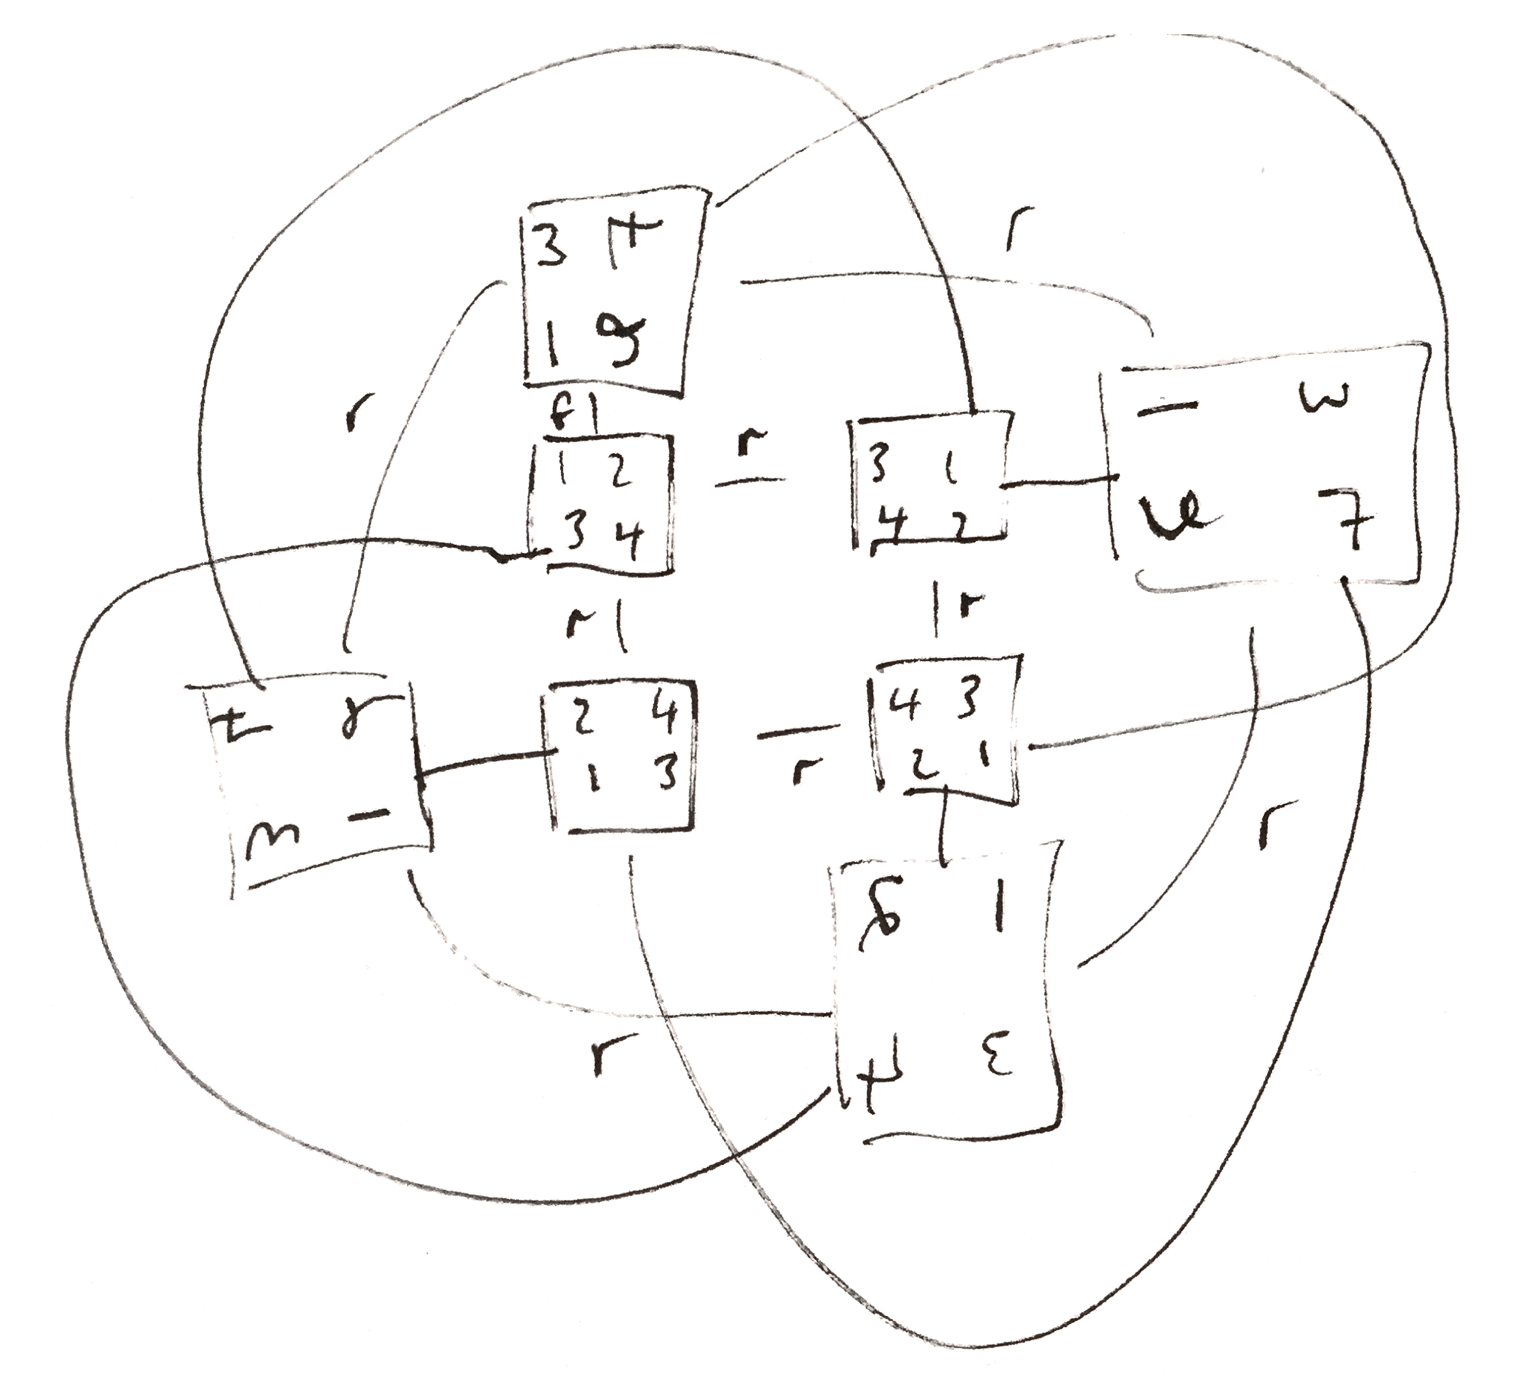
\includegraphics[width=200pt]{img/visual-group-theory-2-8.png}
  \end{mdframed}
  \red{No, this diagram is employing 3 generators when 2 are sufficient. It has a superfluous
    reflection generator.}\\
  $90\deg$ turn ``not allowed'' for reactangle because it does not result in the
  ``same'' rectangle. \checkmark
\item[9] {\bf Show $V_4$ is generated by all pairs of the 3 actions (non-identity elements)}\\
  \begin{mdframed}
    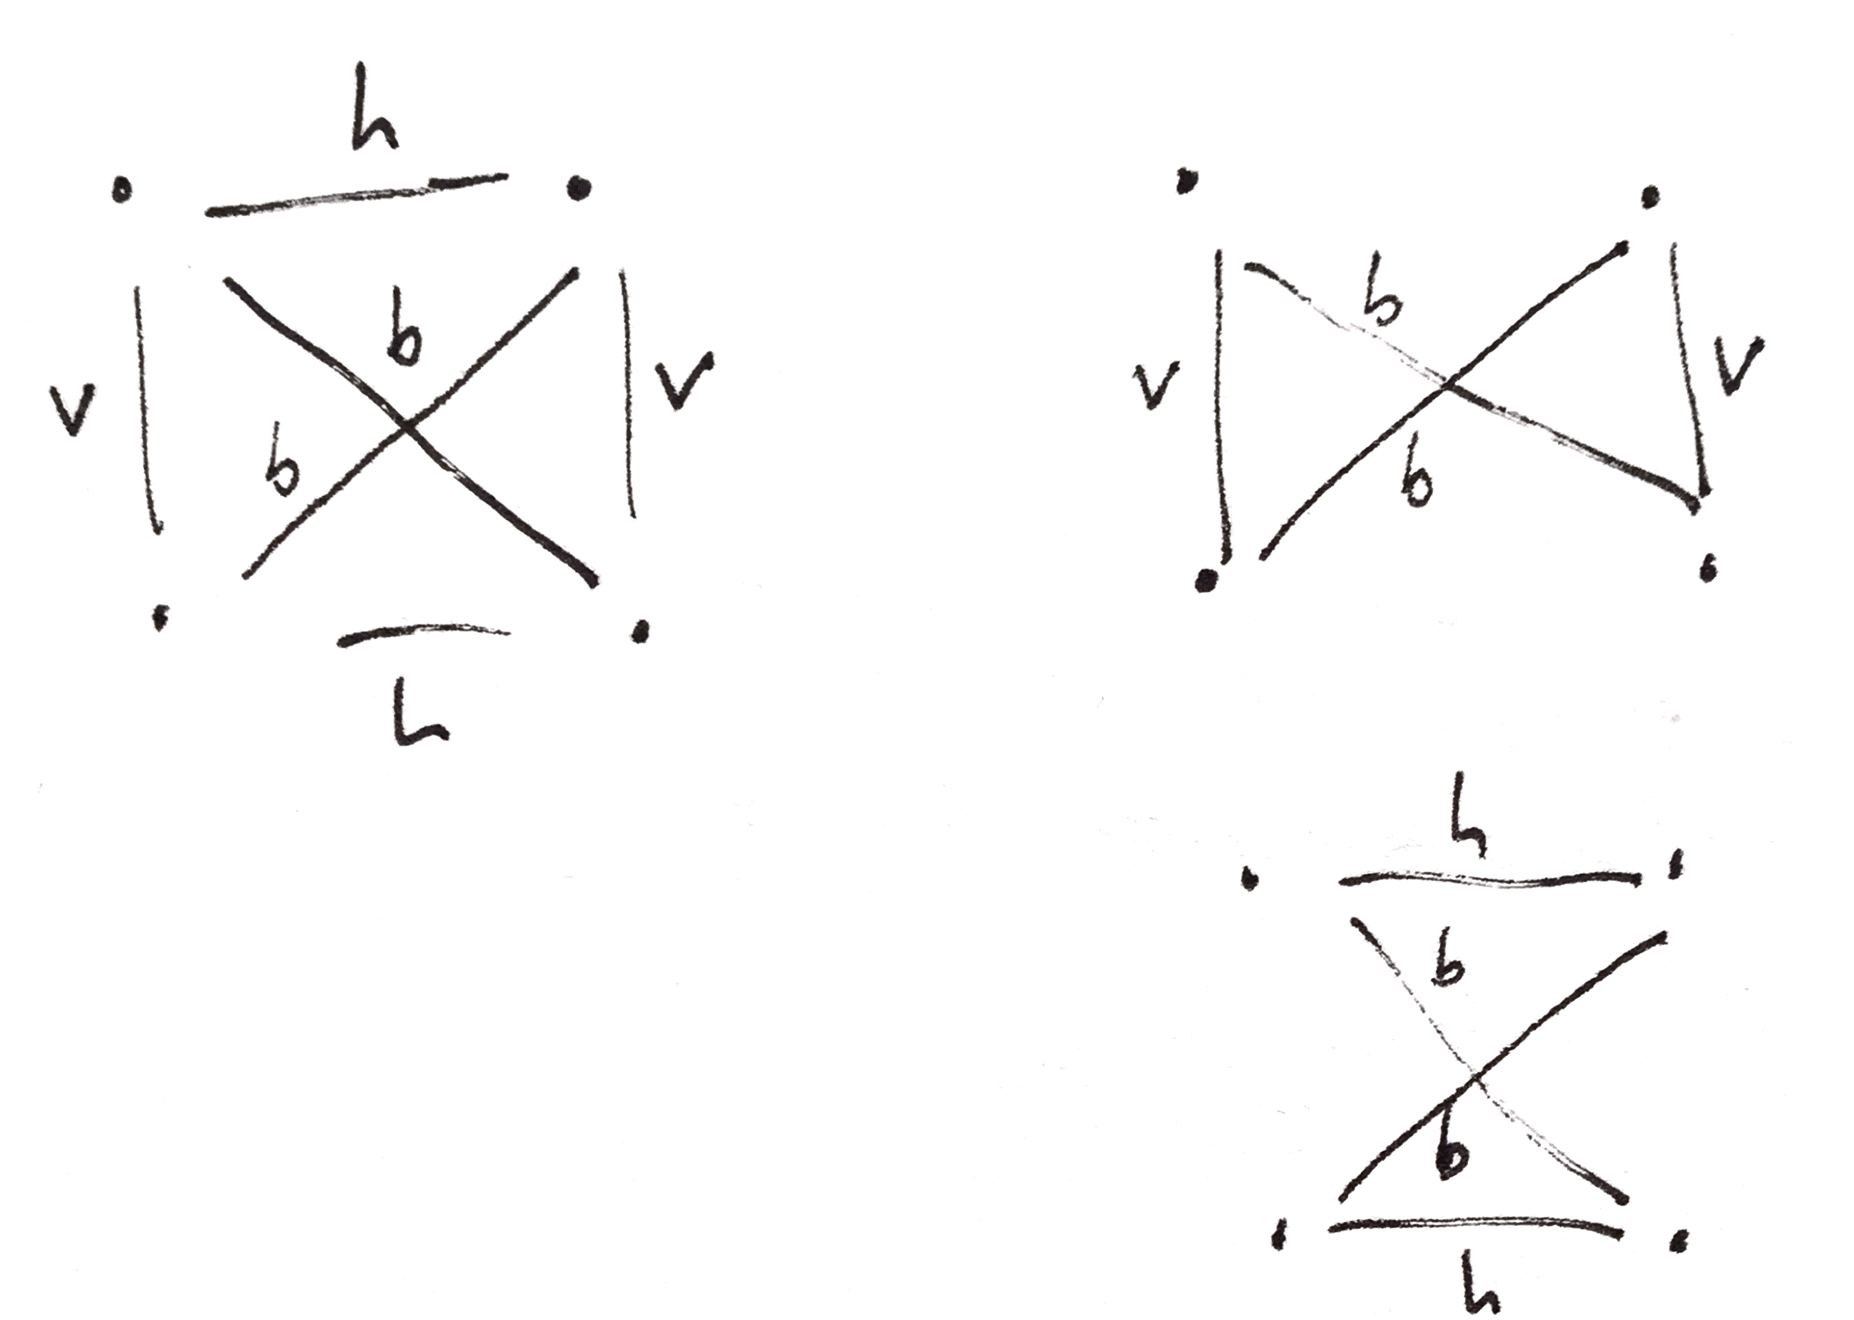
\includegraphics[width=200pt]{img/visual-group-theory-2-9.png}
  \end{mdframed}
  \checkmark
\item[12] {\bf Example of $C_3$}\\
  $\Z/3\Z$, integers under addition mod 3.
\item[13] {\bf Status of generators in Cayley diagram}\\
  arrows represent application of generator elements
\item[15] {\bf If inverse didn't exist}\\
  Some state has no path to initial state, therefore at least one generator arrow must be
  unidirectional.  \red{An element with two arrows pointing to it is irreversible. This corresponds
    to a repeated entry in a row/column of the multiplication table.}
\item[17] {\bf Any sequence of consecutive actions is also an action}\\
  Nodes in a Cayley diagram correspond to actions; if a node is reachable then the sequence of
  generator actions is an action in the group.
\end{enumerate}


\section{}
\begin{enumerate}
\item[6] $Z_4$ \checkmark
\item[8] $D_5$ \checkmark
\item[11] shift L, shift R, reflect H, reflect V?
\item[13] R and L through \checkmark
\end{enumerate}

\section{}
\begin{enumerate}
\item[5] (a) follow two red arows (b) blue then red \checkmark
\item[10a] $A(BB) = Ae = A \neq (AB)B = eB = B$.\\
  $AA = AB = e$ so $A$ has two inverses.
\item[13a] (a)
  $3\cdot 4 = 3$, so 4 acting as identity. \red{not associative}
\item[14] extraneous element \checkmark
\item[17] To get from $g$ to $h$, perform $g^\1h$.
\item[18] latin square
\item[19]
\item[22]
\item[23] smallest noncommutative group is $S_3 = D_3$. \checkmark
\item[24] commutative groups have symmetric multiplication tables
\item[26a] $e^\1 = e$, $a^\1 = a^4$, $(a^2)^\1 = a^3$, $(a^n)^\1 = a^{5 - n}$. \checkmark
\item[27a]
  \begin{align*}
    a^3x &= a^2\\
       x  &= (a^3)^\1a^2 = a^2a^2 = a^4 \checkmark
  \end{align*}
\item[32b] no, lacks inverses \checkmark
\item[33bg] (b) yes \red{zero has no inverse under multiplication} (g) infinite
\end{enumerate}


\section{}
\begin{enumerate}
\item[6c] $D_2$\\
% | e  | r  | f  | fr |
% | r  | e  | fr | f  |
% | f  | fr | e  | r  |
% | fr | f  | r  | e  |
   \begin{center}
    \begin{tabular}{llll}
      e & r & f & fr\\
      r & e & fr & f\\
      f & fr & e & r\\
      fr & f & r & e\\
    \end{tabular}
  \end{center}
\item[9] {\bf What are the orders of the first ten symmetric groups, $S_1$ through $S_{10}$?}
  $1, 2, 6, 24, 120, 720, 5040, 40320, 362880, 3628800$\\
  {\bf Alternating groups}
  $|A_n| =
  \begin{cases}
    \frac{|S_n|}{2}, n > 1\\
    1, n = 1
  \end{cases}.$
  $S_1 = \{e\}$, which is an even permutation, hence $|A_1| = 1$.

\item[20]
\item[23]
\item[24]
\item[28]
\item[30a]
\item[31]
\item[35a]
\item[38]
\item[40a]
\item[43c]
\item[44a]
\end{enumerate}


\section{}
\begin{enumerate}
\item[1]
\item[3a]
\item[12a]
\item[14]
\item[16b]
\item[17d]
\item[23a]
\item[26ab]
\item[28]
\item[30]
\end{enumerate}


\section{}
\begin{enumerate}
\item[3b]
\item[4c]
\item[8]
\item[9]
\item[14ad]
\item[15ad]
\item[16]
\item[18b]
\item[21]
\item[25d]
\item[33abd]
\end{enumerate}


\section{}
\begin{enumerate}
\item[4c]
\item[6]
\item[9c]
\item[11c]
\item[12f]
\item[13]
\item[16]
\item[17ab]
\item[23a]
\item[24]
\item[28]
\item[29bd]
\item[32bcd]
\item[35]
\item[38bc]
\item[42]
\item[43a]
\item[44abd]
\item[45cd]
\item[46a]
\item[47bcegh]
\item[49]
\item[50]
\end{enumerate}



\end{document}
